\chapter{Base Detection and Tracking}\label{chap:base_tracking}
One part of the work is focused on the estimation of the state of the moving platform. In the different phases we have to use different methods to detect and track the base:
\begin{itemize}
\item to be able to find the platform in the minimum amount of time, at the beginning, we need to inspect the area from a very high altitude. From this height we can see just a few features of the moving car and then the pose estimation are noisy. Furthermore we do not have any assumption on the initial condition of the platform, we just know the magnitude of constant forward velocity $|v_{tan}|$, so we do not know before if at a certain time $t$ the car is moving in a straight line or in a curve, we have to estimate it, and this is possible only tracking the platform for several seconds. 
\item after knowing the type of movement and a rough pose estimation of the moving car, we can use these information to improve our state estimation: getting close to the platform without loosing the tracking, starting a more precise measure (base on tag detection), and filtering the measurements with a theoretical model of the movement.
\end{itemize}

\section{From high altitude}
To find the car we assume that the platform is the only white square moving on the arena.
Base on this assumption, we analyze the images from the down looking camera to find a moving white square and calculate its optical flow to predict its future position.
We perform the following passages:
\begin{itemize}
\item threshold the image in order to find the white features.
\item find all the close shapes in the image.
\item select only the shapes with
\begin{itemize}
\item 4 edges
\item convex contour
\item angles between edges close to $\frac{\pi}{2}$
\end{itemize}
\end{itemize}
At this point we have the position of the four corners of all the squares in the image.\\
Now we try to calculate the optical flow of these points through the sequence of images and we track only the points that are moving with a velocity comparable to the one known $v_{tan}$.\\
To perform the optical flow we use the Lucas-Kanade method. %TODO citazione
It assumes that the displacement of the image contents between two nearby frames is small and approximately constant within a neighborhood of the point p under consideration. Thus the optical flow equation can be assumed to hold for all pixels within a window centered at $p$. Namely, the local image flow vector $(V_{x},V_{y})$ must satisfy:

\begin{align}
\begin{split}
I_{x}(q_{1})V_{x}+I_{y}(q_{1})V_{y}=-I_{t}(q_{1})  \\
I_{x}(q_{2})V_{x}+I_{y}(q_{2})V_{y}=-I_{t}(q_{2})  \\
\vdots \\
I_{x}(q_{n})V_{x}+I_{y}(q_{n})V_{y}=-I_{t}(q_{n}) 
\end{split}
\end{align}

Where $q_{1},q_{2},\dots ,q_{n}$ are the pixels inside the window, and $I_{x}(q_{i}),I_{y}(q_{i}),I_{t}(q_{i})$ are the partial derivatives of the image $I$ I with respect to position x, y and time t, evaluated at the point $q_{i}$ and at the current time.\\
These equations can be written in matrix form $Av=b$, where
\begin{align}
A={\begin{bmatrix}I_{x}(q_{1})&I_{y}(q_{1})\\[10pt]I_{x}(q_{2})&I_{y}(q_{2})\\[10pt]\vdots &\vdots \\[10pt]I_{x}(q_{n})&I_{y}(q_{n})\end{bmatrix}},\quad \quad v={\begin{bmatrix}V_{x}\\[10pt]V_{y}\end{bmatrix}},\quad {\mbox{and}}\quad b={\begin{bmatrix}-I_{t}(q_{1})\\[10pt]-I_{t}(q_{2})\\[10pt]\vdots \\[10pt]-I_{t}(q_{n})\end{bmatrix}}
\end{align}

This system has more equations than unknowns and thus it is usually over-determined. The Lucas-Kanade method obtains a compromise solution by the least squares principle. Namely, it solves the $2\times2$ system:
\begin{align}
\begin{split}
A^{T}Av=A^{T}b\\
{\mathrm  {v}}=(A^{T}A)^{{-1}}A^{T}b
\end{split}
\end{align}
\begin{align}
{\begin{bmatrix}V_{x}\\[10pt]V_{y}\end{bmatrix}}={\begin{bmatrix}\sum _{i}I_{x}(q_{i})^{2}&\sum _{i}I_{x}(q_{i})I_{y}(q_{i})\\[10pt]\sum _{i}I_{y}(q_{i})I_{x}(q_{i})&\sum _{i}I_{y}(q_{i})^{2}\end{bmatrix}}^{{-1}}{\begin{bmatrix}-\sum _{i}I_{x}(q_{i})I_{t}(q_{i})\\[10pt]-\sum _{i}I_{y}(q_{i})I_{t}(q_{i})\end{bmatrix}}
\end{align}
With this method we can track the interesting points from frame to frame, calculate direction and velocity of the car and so predict where it will be after a time $t$.\\
\begin{figure}[!htbp]
  \centering
  {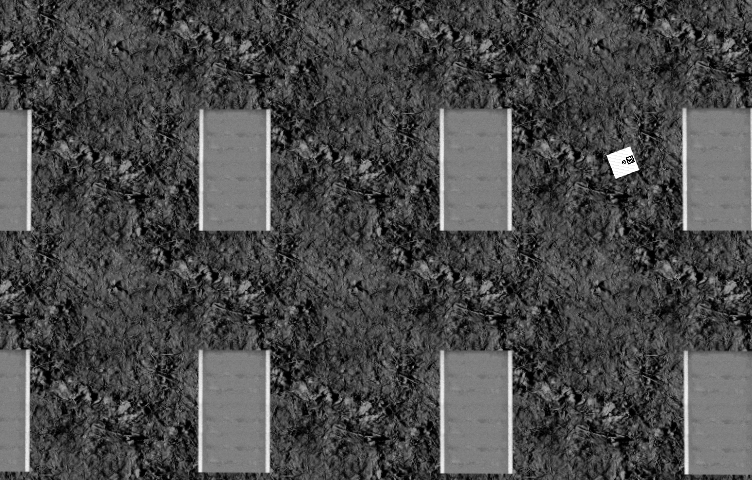
\includegraphics[width=0.45\textwidth]{img/18730previousImage.png}\label{fig:original}}
  \hfill
  {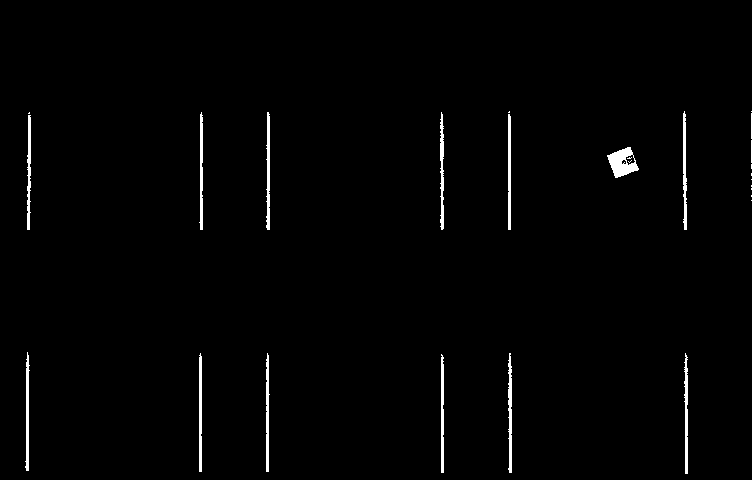
\includegraphics[width=0.45\textwidth]{img/18730_thresholded.png}\label{fig:threshold}}
  \vspace{1cm}
  
  {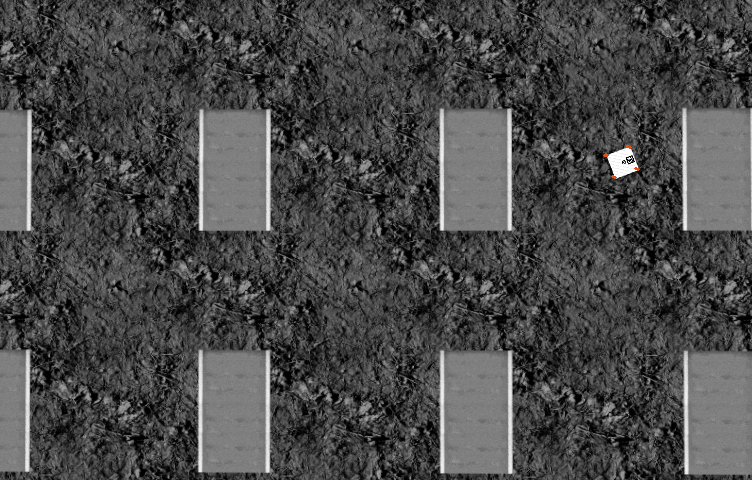
\includegraphics[width=0.45\textwidth]{img/18741_optical_flow.png}\label{fig:optical1}}
  \hfill
  {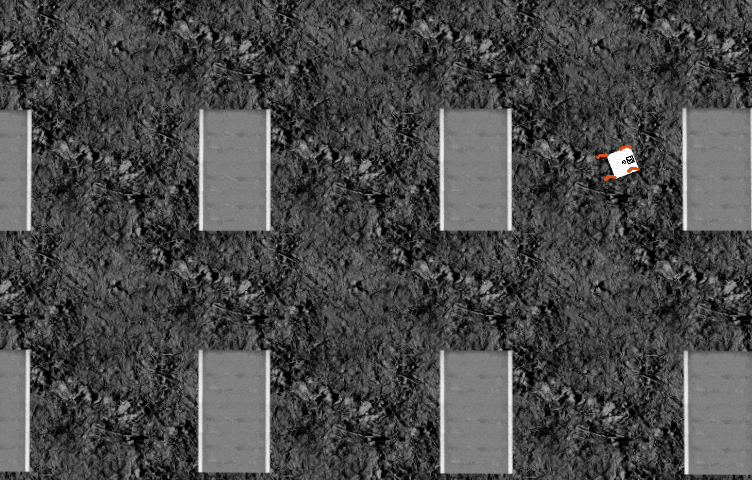
\includegraphics[width=0.45\textwidth]{img/18758_optical_flow.png}\label{fig:optical2}}
  \vspace{1cm}
  
  {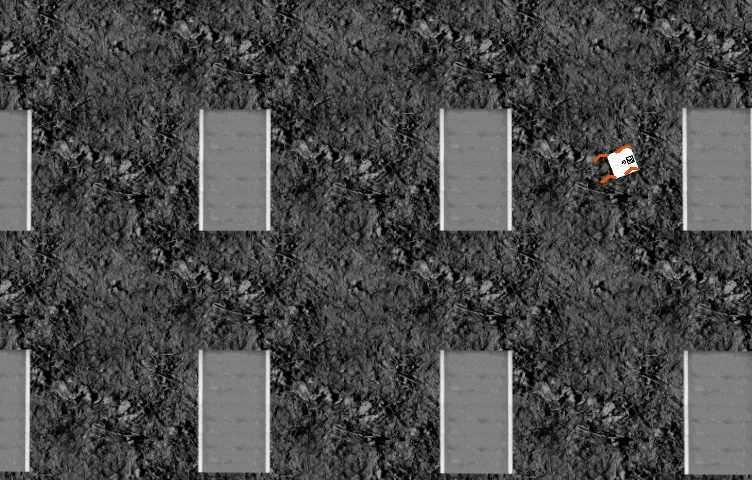
\includegraphics[width=0.45\textwidth]{img/18777_optical_flow.png}\label{fig:optical3}}
  \hfill
  {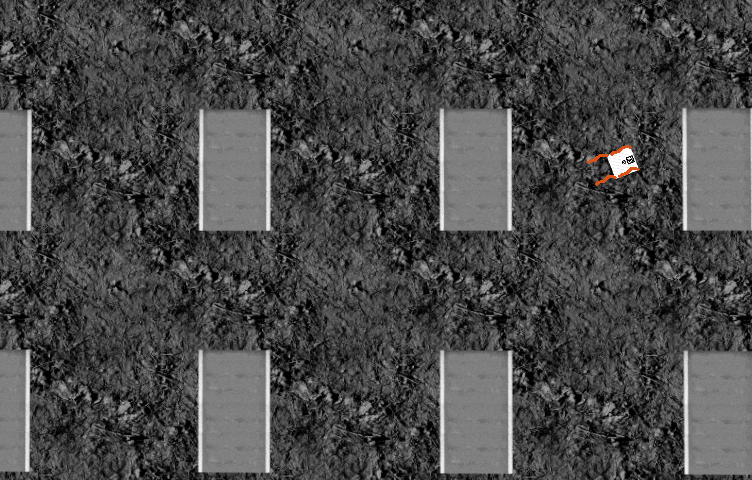
\includegraphics[width=0.45\textwidth]{img/18800_optical_flow.png}\label{fig:optical4}}
   
  \vspace{1cm}
  {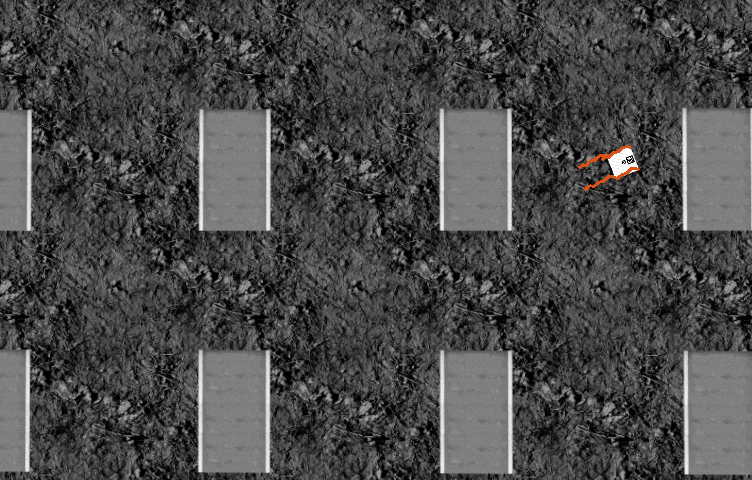
\includegraphics[width=0.45\textwidth]{img/18856_optical_flow.png}\label{fig:optical5}}
  \hfill
  {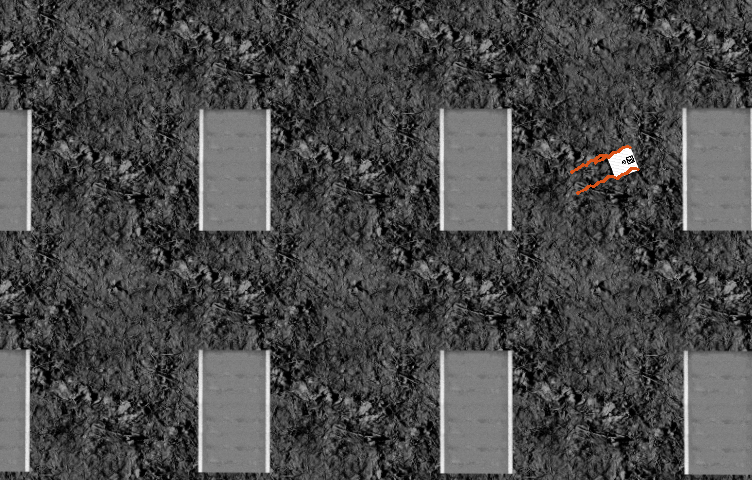
\includegraphics[width=0.45\textwidth]{img/18881_optical_flow.png}\label{fig:optical6}}
 
  \caption{A sequence of images where the moving car is detected and tracked. First image is the original image. Then the one after thresholding. Then all the subsequent images where the corners of the platform are tracked.}
  \label{fig:optical_folw_sequence}
\end{figure} 

\subsubsection{From images to real world}
After tracking the platform in the images, we have to find its position in the 3D real world. This position is calculate using the pinhole model of the camera: %TODO citazione
\begin{align}
wm = A [R|t]M
 \label{eq:pinholemodel}
\end{align}
In expanded form:
\begin{align}
{w\begin{bmatrix}
u \\[10pt]
v  \\[10pt]
1
\end{bmatrix}}=
{\begin{bmatrix}\
f_x & 0 & c_x \\[10pt]
0 & f_y &c_y \\[10pt]
0 & 0 & 1
\end{bmatrix}}
{\begin{bmatrix}\
r_{11} & r_{12} & r_{13} & t_{x} \\[10pt]
r_{21} & r_{22} & r_{23} & t_{y} \\[10pt]
r_{31} & r_{32} & r_{33} & t_{z}
\end{bmatrix}}
{\begin{bmatrix}
X \\[10pt]
Y \\[10pt]
Z \\[10pt]
1
\end{bmatrix}}
\end{align}
Where:
\begin{itemize}
 \item $m$ homogeneous coordinate of the projection point in pixel.
  \item $M$ homogeneous coordinate of a 3D point in the world coordinate frame.
 \item $A$ is the camera matrix or the matrix of intrinsic parameters. It is Composed by $f_x,f_y$ the focal lengths and $c_x,c_y$ the principal point.
 \item $[R|t]$ is the joint rotation-translation matrix or matrix of extrinsic parameters. It express the camera motion around the static scene. This matrix denote the coordinate system transformations from 3D world coordinates to 3D camera coordinates. The position $C$ of the camera expressed in world coordinates is $C=-R^{{-1}}t=-R^{T}t$.
\end{itemize}

We can calculate the depth of the platform using the known dimension of the base: given the length $l_w$ of the square in the real world and the average dimension of the edges in the image $l_i$, we can calculate the depth with respect to the camera frame 
\begin{align}
z = \frac{l_w f}{l_i}
\end{align}
To calculate the dimension $l_i$ we need at least 3 corner of the base and we calculate all the pairwise distances between the corners \ref{fig:platform_profile}:
\begin{itemize}
\item if we have 4 corners there are 6 different distances: 4 of which equal to $l_i$ and 2 $\sqrt{2}l_i$
\item if we have 3 corners there are 3 different distances: 2 of which equal to $l_i$ and 1 $\sqrt{2}l_i$
\end{itemize}
This approximation is not really precise when we see the platform with a camera not perpendicular to the base, but we need just a rough approximation of the height in this first phase.
\begin{figure}[!htbp]
  \centering
  {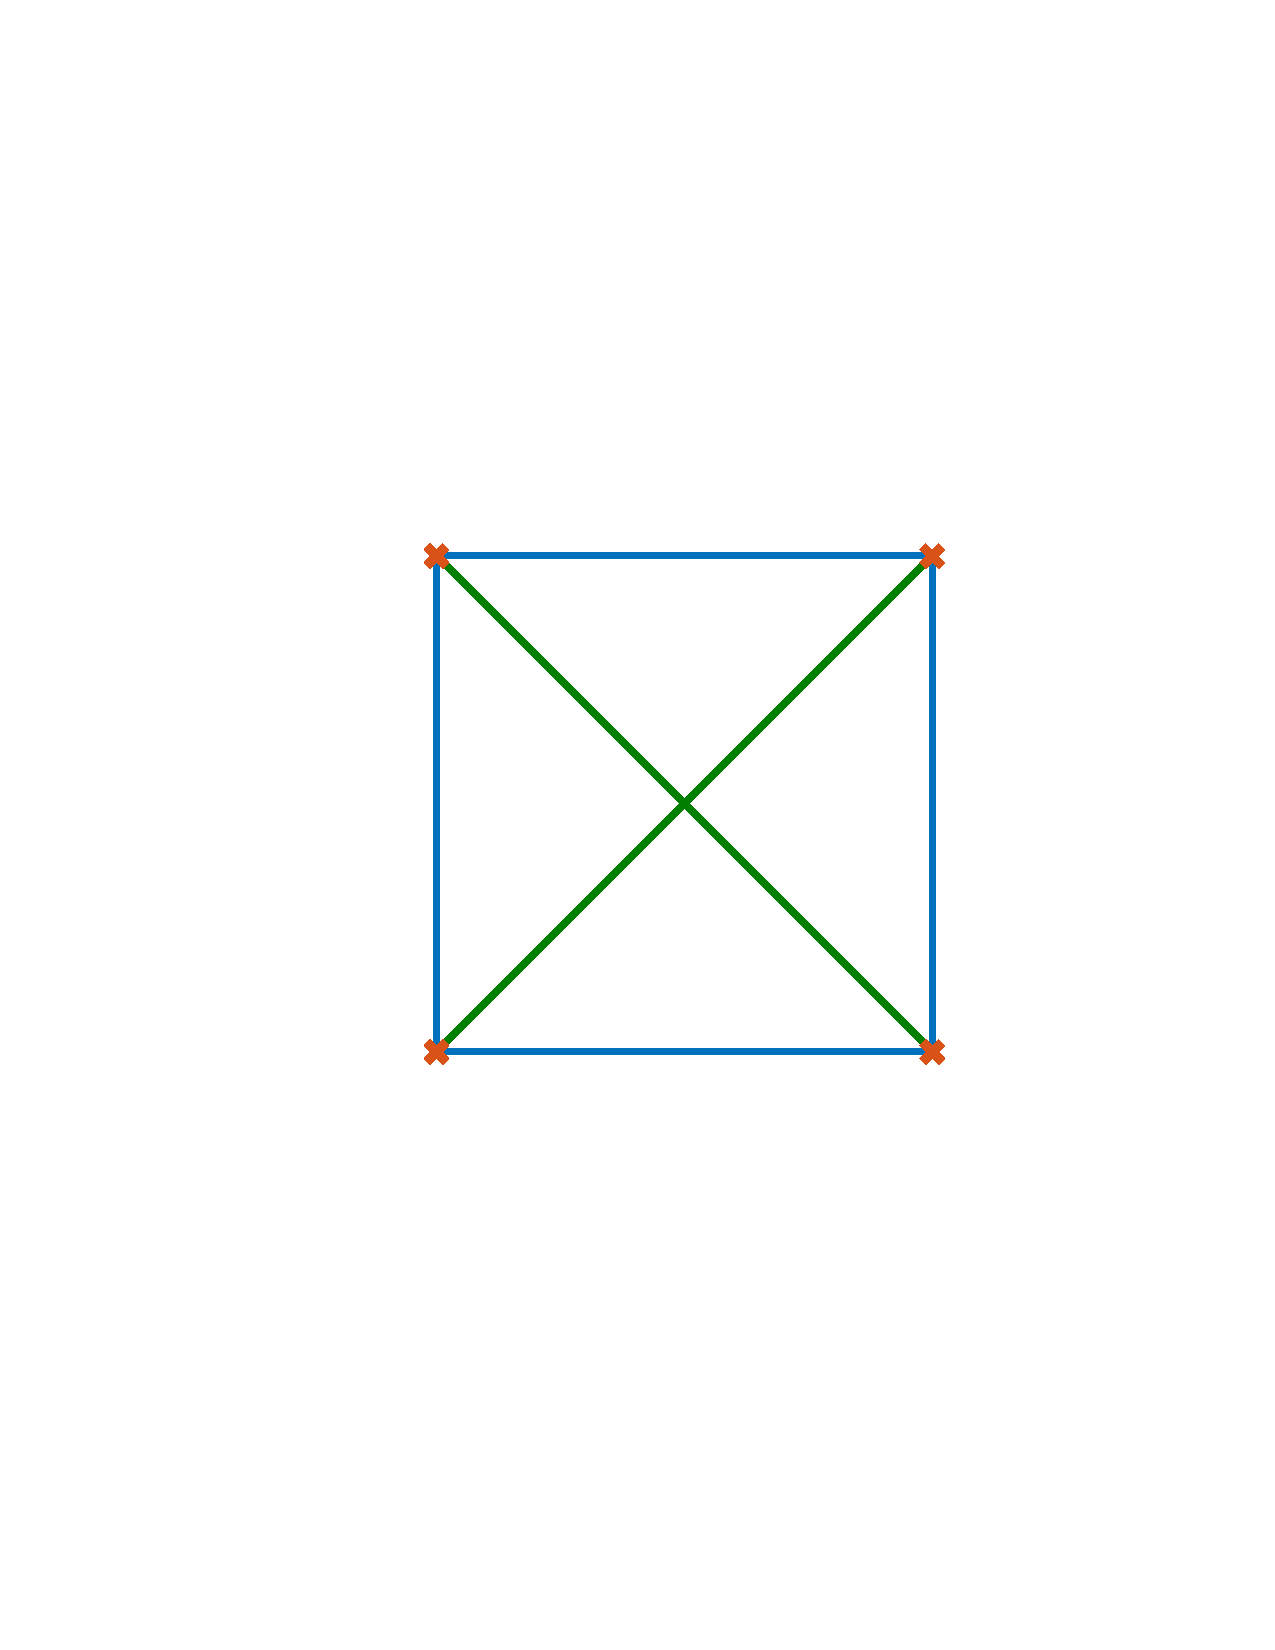
\includegraphics[width=0.3\textwidth]{img/platform_4_edges.pdf}\label{fig:4_corners}}
  \hspace{5em}
  {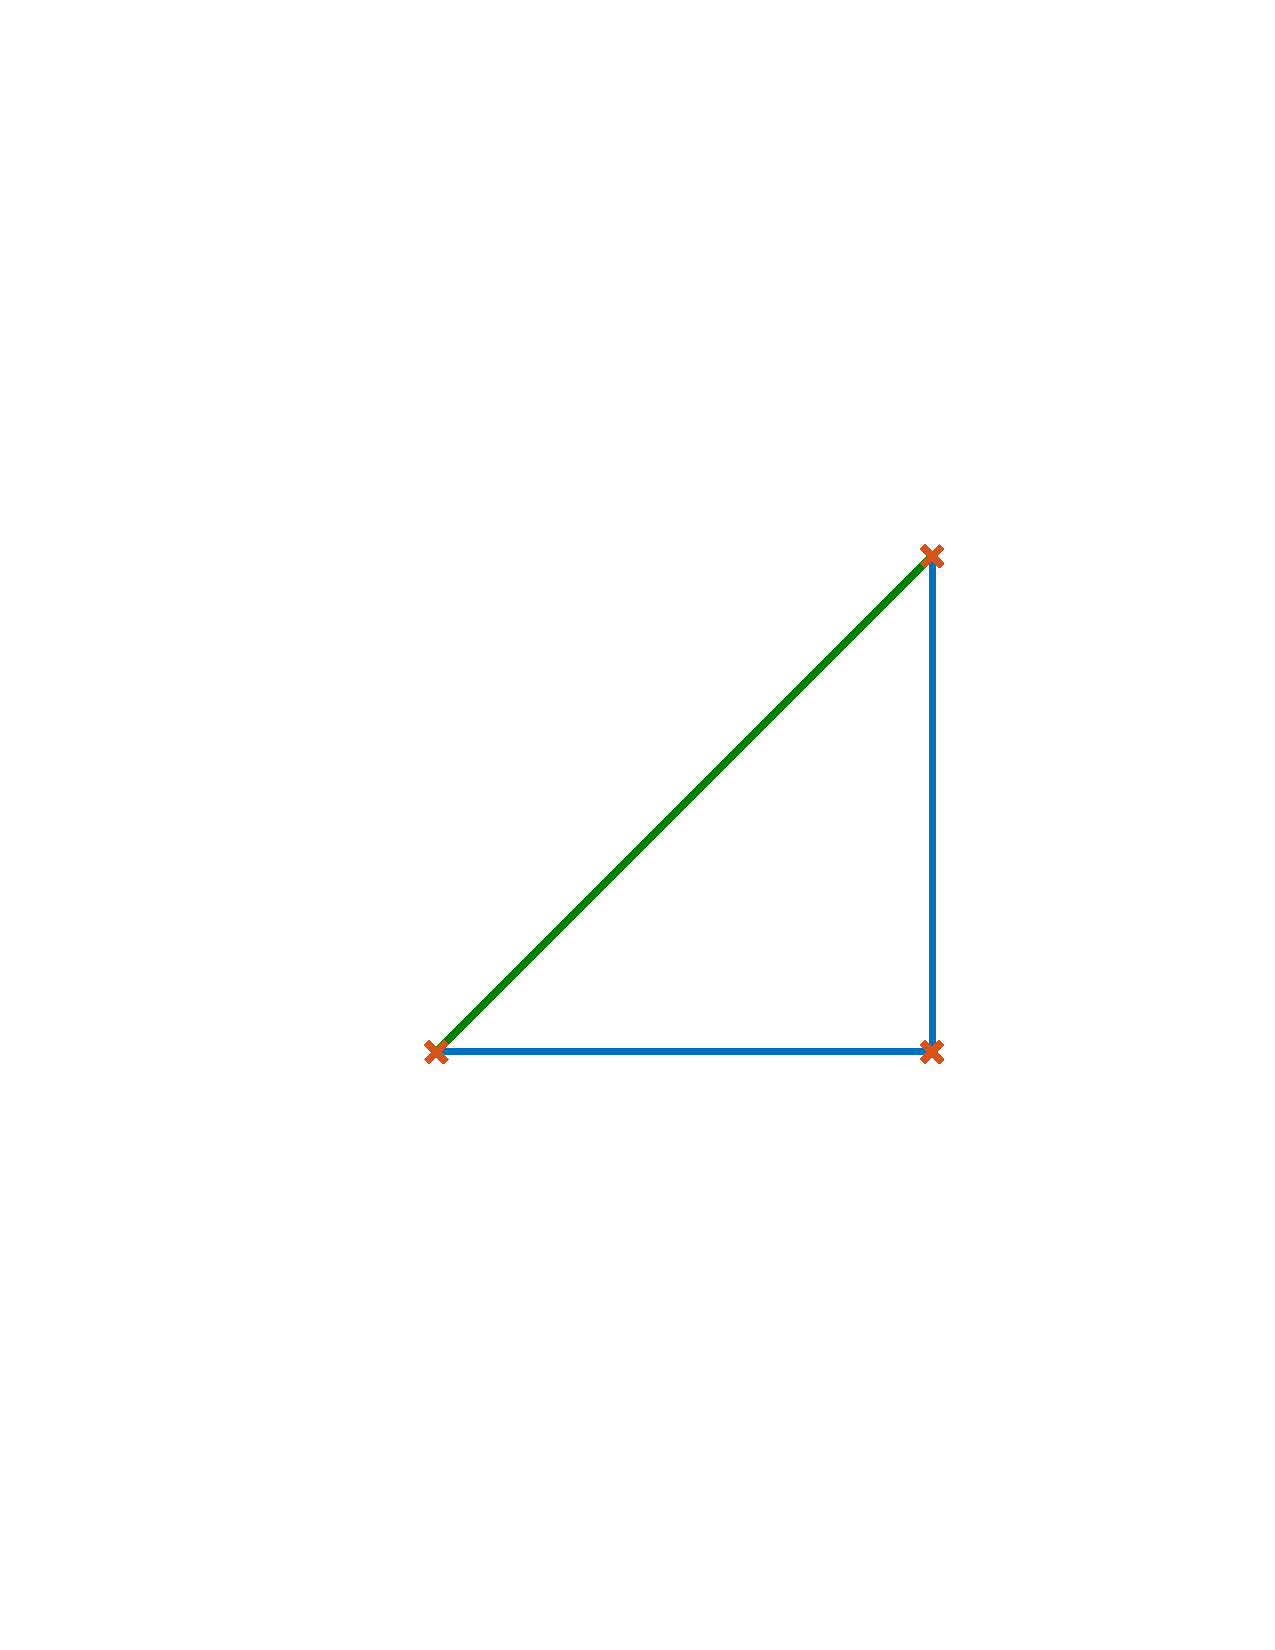
\includegraphics[width=0.3\textwidth]{img/platform_3_edges.pdf}\label{fig:3_corners}}
  \caption{Model of the square platform detected on the image. Red crosses corner detected. Blue lines edges with length $l_i$. Green lines edges with length $\sqrt{2}l_i$ }
  \label{fig:platform_profile}
\end{figure} 

If this depth $z!=0$ we can  solve the system of equation \ref{eq:pinholemodel} finding an unique solution using the following equivalent equations:
\begin{align}
\begin{split}
x &= z\frac{u-c_x}{f_x}\\[10pt]
y &= z\frac{u-c_y}{f_y}\\[10pt]
{\begin{bmatrix}
x \\[10pt]
y \\[10pt]
z
\end{bmatrix}} &= 
R {\begin{bmatrix}
X \\[10pt]
Y \\[10pt]
Z
\end{bmatrix}} + t
\end{split}
\end{align}

A better method to find the position of the platform, without the approximation of the depth $z$ is to resolve a Perspective-n-Point problem %TODO cite
that estimates the pose of a camera given a set of n 3D points in the world and their corresponding 2D projections in the image. The only issue is that to solve this problem without ambiguity the minimum number of points is 4, and sometimes we can track only 3 corners of the base, but when all the 4 points are available we solve the correspondent PnP problem to find a better estimation of the base position.\\

With this method every time we detect the car we can estimate its position and velocity vector in world coordinate frame, so  we can predict where the platform will be in $t$ seconds and where the quadrotor should go to following the base.\\

\section{From low altitude}

\subsection{Extended Kalman Filter}
An Extended Kalman Filter is design in order to have the most reliable value of the state of the platform.

Kalman filtering is an algorithm that uses a series of noisy measurements observed over time and produces estimates of unknown variables that tend to be more precise than those based on a single measurement alone, by using Bayesian inference and estimating a joint probability distribution over the variables for each time frame.\\
The algorithm works in a two-step process:
\begin{itemize}
\item In the prediction step, the Kalman filter produces estimates of the current state variables, along with their uncertainties, based on a model of the system:
\begin{equation}
\boldsymbol{x}_k = f(\boldsymbol{x}_{k-1},\boldsymbol{u}_k) + \boldsymbol{w}_k
\end{equation}
\item Once the outcome of the next measurement is observed:
\begin{equation}
\boldsymbol{z}_k = h(\boldsymbol{x}_{k}) + \boldsymbol{v}_k
\end{equation}
these estimates are updated using a weighted average, with more weight being given to estimates with higher certainty.
\end{itemize}
In the extended Kalman filter, the state transition and observation models don't need to be linear functions of the state but may instead be differentiable functions.\\
($\boldsymbol{w}_k$ and $\boldsymbol{v}_k$ are the process and observation noises which are both assumed to be zero mean multivariate Gaussian noises with covariance $\boldsymbol{Q}_k$ and $\boldsymbol{R}_k$ respectively. $\boldsymbol{u}_k$ is the control vector).

  The algorithm is recursive. It can run in real time, using only the present input measurements and the previously calculated state and its uncertainty matrix; no additional past information is required.\\
The Kalman filter does not require any assumption that the errors are Gaussian. However, the filter yields the exact conditional probability estimate in the special case that all errors are Gaussian-distributed.\\
Initialization
\begin{align}
\begin{split}
\boldsymbol{x}_{0|0} = x_0\\
\boldsymbol{P}_{0|0} = P_0
\end{split}
\end{align}
In this case the prediction equations are continuous in time, so for the prediction step of the EKF we have to solve:
\begin{align}
\begin{split}
\boldsymbol{\dot{\hat{x}}}(t) &= f(\boldsymbol{\hat{x}}(t),\boldsymbol{u}(t)) \\
\boldsymbol{\dot{P}}(t) &= \boldsymbol{F}(t) \boldsymbol{P}(t) + \boldsymbol{P}(t)\boldsymbol{F}(t)^{\top } + \boldsymbol{Q}(t)
\end{split}
\end{align}
for $t \in (t_{k-1}, t_k)$ where %TODO
\begin{align}
\begin{split}
\boldsymbol{\hat{x}}(t_{k-1}) &= \hat{x}_{k-1|k-1} \\
\boldsymbol{P}(t_{k-1}) &= P_{k-1|k-1}
\\
{\boldsymbol{F}}(t)&=\left.{\frac  {\partial f}{\partial {\boldsymbol{x}}}}\right\vert _{{{\hat  {{\boldsymbol{x}}}}(t),{\boldsymbol{u}}(t)}}  \\
\boldsymbol{\hat{x}}_{k|k-1} &= \boldsymbol{\hat{x}}(t_{k}) \\
\boldsymbol{P}_{k|k-1} &= \boldsymbol{P}(t_{k})
\end{split}
\end{align}
In order to save some computation we can discretize the dynamicin order to have shorter computation during the prediction step of the EKF:
\begin{align}
\begin{split}
\boldsymbol{\hat{x}}_{k|k-1} &= f(\boldsymbol{\hat{x}}_{k-1|k-1},\boldsymbol{u}_k) \\
\boldsymbol{P}_{k|k-1} &= \boldsymbol{F}_{k-1} \boldsymbol{P}_{k-1|k-1}\boldsymbol{F}_{k-1}^{\top } + \boldsymbol{Q}_{k}
\end{split}
\end{align}
where the state transition matrix is defined to be the following Jacobians:
\begin{align}
\begin{split}
\boldsymbol{F}_{k-1}&= \left.{\frac{\partial f}{\partial {\boldsymbol{x}}}} \right \vert_{\hat{\boldsymbol{x}}_{k-1|k-1},\boldsymbol{u}_{k}} 
\end{split}
\end{align}
While the update equations are discrete in time and they yield to the following update step: 
\begin{align}
\begin{split}
\boldsymbol{K}_{k} &= \boldsymbol{P}_{k|k-1} \boldsymbol{H}_{k}^{\top }(\boldsymbol{H}_{k} \boldsymbol{P}_{k|k-1} \boldsymbol{H}_{k}^{\top }+ \boldsymbol{R}_{k})^{-1}
\\
\hat{\boldsymbol{x}}_{k|k} &= \hat{\boldsymbol{x}}_{k|k-1} + \boldsymbol{K}_{k} (\boldsymbol{z}_{k}-h(\hat{\boldsymbol{x}}_{k|k-1}))
\\
\boldsymbol{P}_{k|k} &=(\boldsymbol{I}-\boldsymbol{K}_{k}\boldsymbol{H}_{k})\boldsymbol{P}_{k|k-1}
\end{split}
\end{align}
where the observation matrix is defined to be the following Jacobian:

\begin{align}
\begin{split}
\boldsymbol{H}_{k} = \left.{\frac{\partial h}{\partial {\boldsymbol{x}}}} \right \vert_{\hat{\boldsymbol{x}}_{k|k-1}}
\end{split}
\end{align}

\subsubsection{Prediction update: non-holonomic model}
The platform is considered as a car and simulated with a non-holonomic model. 
In this model the state is defined as $\boldsymbol{x} = (x, y, z,\theta , v, \phi)$:
It corresponds to the 3 position in a space $(x,y,z)$ and the yaw angle of the platform $(\theta)$ w.r.t. the world frame, the forward velocity ($v$) and the angle of the front wheels ($\phi$). The system depends on a parameter $L$ that corresponds to the distance between the front and the back wheels.\\
In this model the control input are the change in velocity $v$ and in the angle of curvature $\phi$. \\
The equation of motion in continuous time are:
\begin{align}
\boldsymbol{\dot{x}} = f(\boldsymbol{x},\boldsymbol{u}) \nonumber
\end{align}
\begin{align}
\begin{split}
\dot{x} &= v cos(\theta) \\
\dot{y} &= v sin(\theta) \\
\dot{z} &= 0 \\
\dot{\theta} &= \frac{v}{L}tan(\phi)\\
\dot{v} &= u_1 \\
\dot{\phi} &= u_2 
\end{split}
\end{align}
It is possible to discretize these dynamics in $t \in (t_{k-1}, t_k)$ with a first order finite difference:
\begin{align}
\boldsymbol{\dot{x}} \approx \frac{\boldsymbol{x}_k - \boldsymbol{x}_{k-1} }{dt} \approx f(\boldsymbol{x}_{k-1},\boldsymbol{u}_k) \nonumber
\end{align}
with $\boldsymbol{x}_k = \boldsymbol{x}(t_k)$, $\boldsymbol{x}_{k-1} = \boldsymbol{x}(t_{k-1})$, $dt = t_k - t_{k-1}$
\begin{align}
\begin{split}
x_k &= x_{k-1} + dt \big(v_{k-1} cos(\theta_{k-1})\big) \\
y_k &= y_{k-1} + dt \big(v_{k-1} sin(\theta_{k-1})\big) \\
z_k &= z_{k-1} \\
\theta_k &= \theta_{k-1} + dt\Big(\frac{v_{k-1}}{L}tan(\phi_{k-1}) \Big)\\
v_{k} &= v_{k-1} + dt \big(u_{1k}\big) \\
\phi_k &= \phi_{k-1} + dt \big(u_{2k}\big) 
\end{split}
\end{align}
In order to solve the former system, we have anyway to find a numerical solution. For this purpose we use a    
RUNGE-KUTTA scheme %TODO
\begin{figure}[!ht]
    \centering
    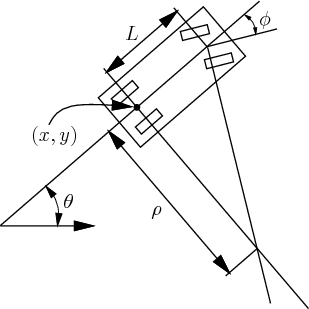
\includegraphics[width=0.5\textwidth]{img/non_holonomic_model.png}
    \caption{Non-holonomic model}
    \label{fig:nonholonomicmodel}
\end{figure}
\paragraph{Straight and circular path}
For now we assume the input $u_1$ and $u_2$  are equal to zero, so the platform can be static ($v_f(0) = 0$) can move in a straight line ($v_f(0) \neq 0$ and $\phi(0) = 0$) or in a circle ($v_f(0) \neq 0$ and $\phi(0) \neq 0$)


\subsection{Measurement update}
\subsubsection{Tag Detector}

\paragraph{April Tag vs Ar Sys}
precision comparison vs frequency
nodlet
\subsubsection{Cross Detector}
pnp problem
\subsubsection{Covariance Estimation}



\section{Results}
\begin{figure}[!ht]
    \centering
    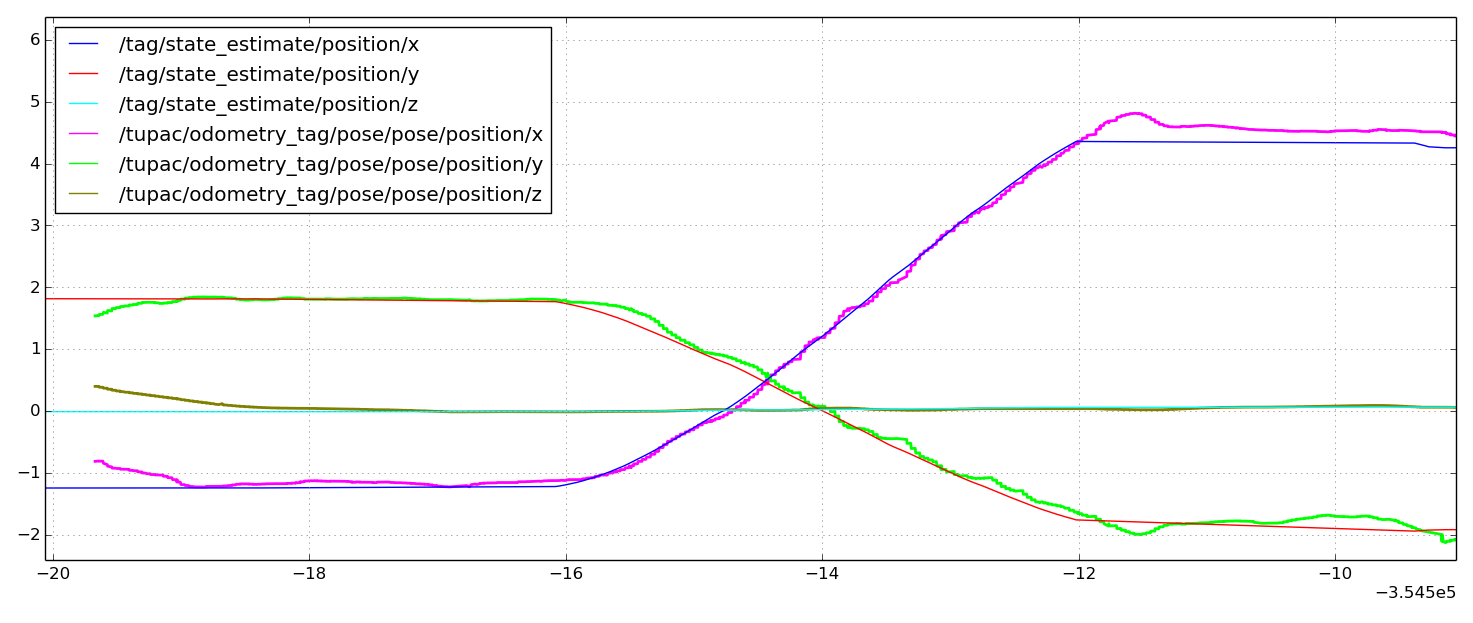
\includegraphics[width=0.97\textwidth]{img/position_real_world_fast.png}
    \caption{EKF 1}
    \label{fig:ekf_position_fast}
\end{figure}
\begin{figure}[!ht]
    \centering
    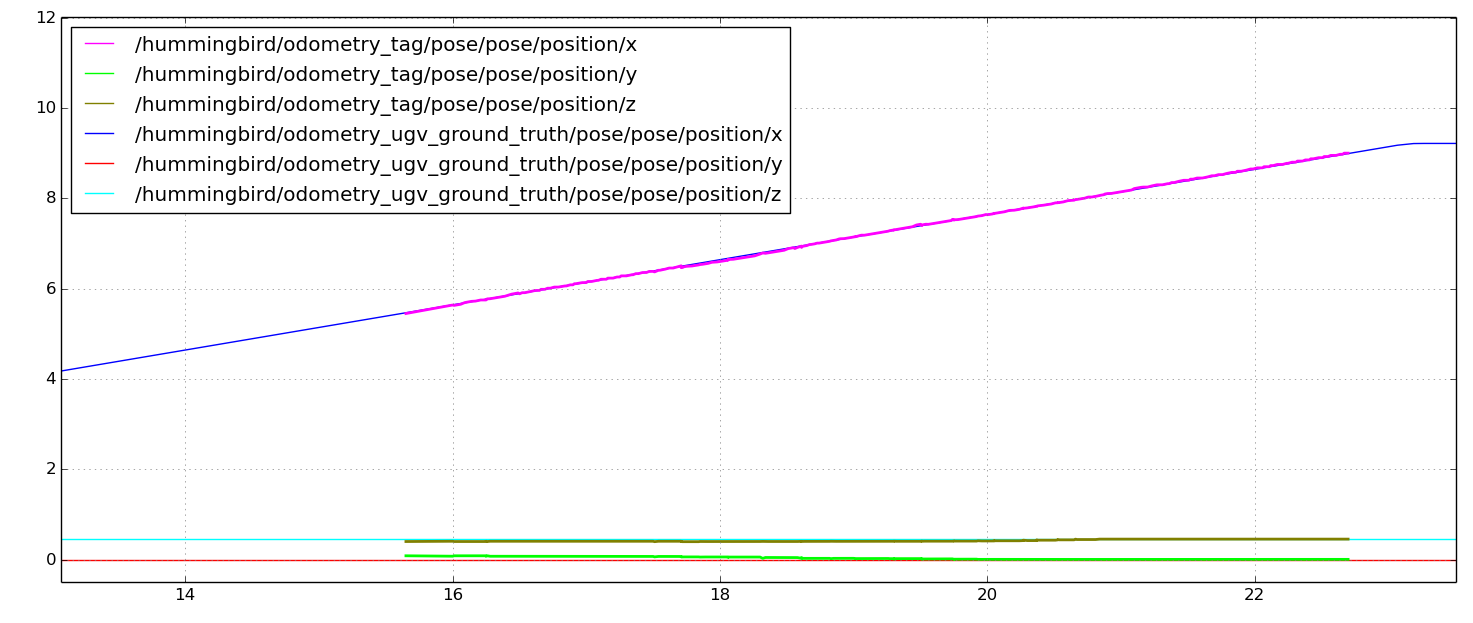
\includegraphics[width=0.97\textwidth]{img/position_simulation_hot_init.png}
    \caption{EKF 2}
    \label{fig:ekf_position_hot_init}
\end{figure}
